\begin{figure*}[t]
\label{fig:kv_cache_summary}
\centering
\tikzset{
    basic/.style  = {draw, text width=2cm, align=center, font=\sffamily, rectangle},
    root/.style   = {basic, rounded corners=2pt, thin, align=center, fill=white,text width=8cm, rotate=90, font=\footnotesize},
    dnode/.style = {basic, thin, rounded corners=2pt, align=center, fill=nblue,text width=3.5cm, font=\footnotesize},
    dnode_1/.style = {basic, thin, rounded corners=2pt, align=center, fill=nblue,text width=2cm, font=\footnotesize},
    dnode_2/.style = {basic, thin, rounded corners=2pt, align=center, fill=nblue,text width=1.7cm, font=\footnotesize},
    mnode/.style = {basic, thin, rounded corners=2pt, align=center, fill=blue!10,text width=3.5cm, font=\footnotesize},
    mnode_1/.style = {basic, thin, rounded corners=2pt, align=center, fill=blue!10,text width=2cm, font=\footnotesize}, 
    snode/.style = {basic, thin, rounded corners=2pt, align=center, fill=npurple,text width=3.5cm, font=\footnotesize},
    snode_1/.style = {basic, thin, rounded corners=2pt, align=center, fill=npurple,text width=2cm, font=\footnotesize},
    tnode/.style = {basic, thin, align=left, fill=pink!60, text width=15em, align=center},
    xnode/.style = {basic, thin, rounded corners=2pt, align=center, fill=blue!20,text width=5cm,},
    wnode/.style = {basic, thin, rounded corners=2pt, align=left, fill=white,text width=5.8cm, font=\footnotesize},
    wnode_1/.style = {basic, thin, rounded corners=2pt, align=left, fill=white,text width=5cm, font=\footnotesize},
    wnode_2/.style = {basic, thin, rounded corners=2pt, align=left, fill=white,text width=6cm, font=\footnotesize},
    %edge from parent/.style = {draw=black, edge from parent fork right}
    %edge from parent/.style = {draw=black, edge from parent fork down}
}
%
\begin{forest} 
for tree={
    grow=east,
    growth parent anchor=east,
    parent anchor=east,
    child anchor=west,
    edge path={\noexpand\path[\forestoption{edge},->, >={latex}] 
         (!u.parent anchor) -- +(5pt,0pt) |- (.child anchor)
         \forestoption{edge label};}
}
% l sep is used for arrow distance
[Token-level Optimization, dnode_2
    [KV Cache Low-rank Decomposition  (Sec.~\ref{ssec:kv_low_rank}), dnode
            [Learned Low-rank Approximation  (Sec~\ref{sssec:kv_low_rank_learned}), dnode
                [   
                    {LESS~\cite{dong2024get},
                    MatryoshkaKV~\cite{linMatryoshkaKVAdaptiveKV2024}
                    }, wnode_1
                ]
            ]
            [Tensor\\ Decomposition  (Sec~\ref{sssec:kv_low_rank_tensor}), dnode
                [
                    {DecoQuant~\cite{liu2024unlocking}
                    }, wnode_1
                ]            
            ]
            [Singular Value Decomposition  (Sec~\ref{sssec:kv_low_rank_svd}), dnode
                [
                    {ECKVH~\cite{yu2024effectively}, EigenAttention~\cite{saxena2024eigen}, 
                    ZDC~\cite{zhang2024zero}, 
                    LoRC~\cite{zhang2024lorc},
                    ShadowKV~\cite{sun2024shadowkv},
                    Palu~\cite{chang2024palu} 
                    }, wnode_1
                ]
            ]
        ]
         [KV Cache \\Quantization  (Sec.~\ref{ssec:kv_quant}), dnode
            [Outlier Redistribution  (Sec~\ref{sssec:outlier_redistribution}), dnode
                [
                {MassiveActivation~\cite{DBLP:journals/corr/abs-2402-17762},
                QuaRot~\cite{ashkboos2024quarot}, Qserve~\cite{DBLP:journals/corr/abs-2405-04532},  Q-INT4~\cite{DBLP:conf/nips/XiLCZ23},
                SpinQuant~\cite{liu2024spinquant},
                DuQuant~\cite{lin2024duquant},
                SmoothQuant~\cite{DBLP:conf/icml/XiaoLSWDH23},
                OS+~\cite{wei2023outlier},
                 AffineQuant~\cite{ma2024affinequant},
                 FlatQuant~\cite{sun2024flatquant},
                 AWQ~\cite{DBLP:conf/mlsys/0002TTYCWXDG024},
                OmniQuant~\cite{shao2023omniquant} }, wnode_1
                ]
            ]
            [Mixed-precision Quantization  (Sec~\ref{sssec:kv_quant_mixed_precision}), dnode
                [
                    {
                    KVQuant~\cite{hooper2024kvquant},
                    IntactKV~\cite{liu2024intactkv},
                    SKVQ~\cite{duanmu2024skvq},
                    KIVI~\cite{liu2024kivi},
                    WKVQuant~\cite{yue2024wkvquant},
                    GEAR~\cite{kang2024gear}, 
                    MiKV~\cite{yang2024no}, 
                    ZIPVL~\cite{he2024zipvl},  ZipCache~\cite{he2024zipcache},
                    PrefixQuant~\cite{chen2024prefixquant},
                    MiniKV~\cite{sharma2024minikvpushinglimitsllm}
                 }, wnode_1
                ]
            ]
            [Fixed-precision Quantization  (Sec~\ref{sssec:kv_quant_fixed_precision}), dnode
                [
                    {ZeroQuant~\cite{yao2022zeroquant},
                    FlexGen~\cite{DBLP:conf/icml/0007ZYLRCLRSZ23}, QJL~\cite{zandieh2024qjl},
                    PQCache~\cite{zhang2024pqcache}
                }, wnode_1
                ]
            ]
        ]
        [KV Cache \\Merging  (Sec.~\ref{ssec:kv_merge}), dnode
            [Cross-layer Merging  (Sec~\ref{sssec:kv_merge_cross_layer}), dnode
            [
            {MiniCache~\cite{DBLP:journals/corr/abs-2405-14366}, KVSharer~\cite{yang2024kvsharerefficientinferencelayerwise}},wnode_1
            ]
            ]
            [Intra-layer \\Merging  (Sec~\ref{sssec:kv_merge_intra_layer}), dnode
                [
                {CCM~\cite{DBLP:conf/iclr/KimYYS24},
                LoMA \cite{wangLoMALosslessCompressed2024},
                {DMC}~\cite{nawrotDynamicMemoryCompression2024}, 
                CaM~\cite{DBLP:conf/icml/0002DLZ00J24}, 
                D2O~\cite{DBLP:journals/corr/abs-2406-13035},
                AIM~\cite{zhong2024aim},
                Look-M~\cite{DBLP:conf/emnlp/WanWLHZJW024},
                KVMerger~\cite{DBLP:journals/corr/abs-2407-08454},
                {CHAI}~\cite{agarwalCHAIClusteredHead2024}}, wnode_1
                ]
            ]
        ]
        [KV Cache Budget  Allocation  (Sec.~\ref{ssec:kv_budget}), dnode
            [Head-wise Budget Allocation  (Sec~\ref{sssec:kv_budget_head_wise}), dnode
                [
                {AdaKV~\cite{DBLP:journals/corr/abs-2407-11550}, CriticalKV~\cite{anonymous2024identify}, LeanKV~\cite{zhang2024unifyingkvcachecompression},
                RazorAttention~\cite{DBLP:journals/corr/abs-2407-15891},
                HeadKV~\cite{DBLP:journals/corr/abs-2410-19258},
                DuoAttention~\cite{DBLP:journals/corr/abs-2410-10819}
                },wnode_1
                ]
            ]
            [Layer-wise Budget Allocation  (Sec~\ref{sssec:kv_budget_layer_wise}), dnode
                [
                {PyramidKV~\cite{DBLP:journals/corr/abs-2406-02069}, PyramidInfer~\cite{DBLP:conf/acl/YangHGHZ024}, 
                DynamicKV~\cite{anonymous2024dynamickv}, PrefixKV~\cite{wang2024prefixkvadaptiveprefixkv},
                SimLayerKV~\cite{DBLP:journals/corr/abs-2410-13846}
                }, wnode_1
                ]
            ]
        ]
    [KV Cache \\Selection  (Sec.~\ref{ssec:cache_sel}),dnode
        [Dynamic Selection without Permanent Eviction  (Sec~\ref{sssec:dynamic_kv_no_permanent}), dnode
            [            {InfLLM~\cite{xiao2024infllmtrainingfreelongcontextextrapolation}, Quest~\cite{DBLP:conf/icml/TangZZXKH24}, PQCache~\cite{zhang2024pqcache}, SqueezedAttention~\cite{hooper2024squeezedattentionacceleratinglong}, RetrievalAttention~\cite{DBLP:journals/corr/abs-2409-10516}, 
            EM-LLM~\cite{DBLP:journals/corr/abs-2407-09450}}, wnode_1
            ]
        ]
        [Dynamic Selection with Permanent Eviction  (Sec~\ref{sssec:dynamic_kv_permanent}), dnode
            [ {H2O~\cite{DBLP:conf/nips/Zhang00CZC0TRBW23}, BUZZ~\cite{zhao2024buzzbeehivestructuredsparsekv}, 
            NACL~\cite{DBLP:journals/corr/abs-2408-03675}, Scissorhands~\cite{DBLP:conf/nips/LiuDLWXXKS23}, Keyformer~\cite{DBLP:conf/mlsys/AdnanAJNSK24},
            SepLLM~\cite{chen2024sepllm}},wnode_1
            ]
        ]
        [Static KV Cache Selection  (Sec~\ref{sssec:static_kv}), dnode
            [{FastGen~\cite{DBLP:conf/iclr/Ge0LZ0024}, SnapKV~\cite{li2024snapkv}, Attention-Gate~\cite{DBLP:journals/corr/abs-2410-12876}},wnode_1
            ]
        ]
    ]
]
\end{forest}

\caption{Taxonomy of the Token-level Optimization for KV Cache Management.}
\label{fig:token_framework}
\end{figure*}

\section{Token-level Optimization }
\label{sec:token_level}
In the token level, optimization focuses exclusively on improving KV cache based on the characteristics and patterns of KV pairs of tokens, without considering enhancements from model architecture improvements or system parallelization techniques.
In general, token-level optimization methods are primarily guided by observations from LLMs and sequential inputs. 
Existing approaches can be categorized into five main types: KV cache selection, KV cache budget allocation, KV cache merging, KV cache quantization, and KV cache low-rank decomposition.
The taxonomy of the token-level optimization is shown in Fig.~\ref{fig:token_framework}.

\subsection{KV Cache Selection}\label{ssec:cache_sel}


KV cache selection mechanisms have emerged as a critical optimization strategy, aimed at reducing memory 
utilization of KV caches, minimizing inference latency, and enhancing overall throughput in large language models. 
These optimization objectives have driven the development of various selection methodologies, which can be 
classified into two distinct categories:
(1) \textbf{static KV cache selection}, which performs token filtering exclusively during the prefilling phase, with selected 
tokens remaining fixed throughout subsequent decoding steps; and (2) \textbf{dynamic KV cache selection}, which continuously 
updates KV cache during the decoding phase, enabling adaptive cache management.
In dynamic KV cache selection approaches, KV cache tokens that are not selected may be permanently evicted or offloaded to hierarchical caching devices such as 
CPU memory, implementing a multi-tier storage strategy. 
Given that real-time KV cache selection during decoding may incur substantial computational overhead, 
several studies have focused on developing optimized retrieval algorithms to enhance the efficiency of 
this process. These optimizations include block-level retrieval instead of token-level granularity to reduce 
search complexity, asynchronous query mechanisms to hide latency, and parallel retrieval pipelines to 
accelerate the selection process. These optimization efforts aim to mitigate the computational burden 
while maintaining the effectiveness of token selection.
The summary of the KV cache selection is listed in Tab.~\ref{tab:kv_cache_summary}.


\begin{table*}[ht]
    \centering
    \caption{Comparison of KV cache selection strategies.}
    \label{tab:kv_cache_summary}
    \renewcommand{\arraystretch}{1.3} % 调整行间距
    \setlength{\tabcolsep}{3pt} % 减小列间距
    \begin{tabular}{lccccccc}
        \toprule
        \textbf{Method} & 
        \makecell{\textbf{Initial}\\\textbf{tokens}} & 
        \makecell{\textbf{Top-$k$}\\\textbf{tokens}} & 
        \makecell{\textbf{Recent}\\\textbf{tokens}} & 
        \makecell{\textbf{Permanent}\\\textbf{eviction}} & 
        \makecell{\textbf{Dynamic}\\\textbf{selection}} & 
        \makecell{\textbf{Selection}\\\textbf{granularity}} & 
        \makecell{\textbf{Remark}} \\ 
        \midrule
        %% Prefilling phase
        FastGen~\cite{DBLP:conf/iclr/Ge0LZ0024} & \checkmark & \checkmark & \checkmark & \checkmark  &  & token & five attention structures\\
        SnapKV~\cite{li2024snapkv} &  & \checkmark & \checkmark & \checkmark &  & token & observation window-based\\
        Attention-Gate~\cite{DBLP:journals/corr/abs-2410-12876} & & \checkmark &  & \checkmark &  & token & learned eviction policy\\
        
        %% Decoding phase
        StreamingLLM~\cite{DBLP:conf/iclr/XiaoTCHL24} & \checkmark & & \checkmark & \checkmark  & \checkmark & token & initial and recent tokens \\
        LM-Infinite~\cite{DBLP:conf/naacl/HanWPX0JW24} & \checkmark  & & \checkmark & \checkmark & \checkmark & token & distance ceiling \\
        H2O~\cite{DBLP:conf/nips/Zhang00CZC0TRBW23} & & \checkmark & \checkmark & \checkmark & \checkmark & token &  accmulative attention score \\
        BUZZ~\cite{zhao2024buzzbeehivestructuredsparsekv} & \checkmark & \checkmark & \checkmark & \checkmark & \checkmark & token &  beehive-like structure \\
        Scissorhands~\cite{DBLP:conf/nips/LiuDLWXXKS23} & & \checkmark & \checkmark & \checkmark  & \checkmark & token & persistence of importance \\
        NACL~\cite{DBLP:journals/corr/abs-2408-03675} & & \checkmark & \checkmark & \checkmark & \checkmark & token & diversified random eviction \\
        Keyformer~\cite{DBLP:conf/mlsys/AdnanAJNSK24} & & \checkmark & \checkmark & \checkmark & \checkmark & token & gumbel logit adjustment \\

        %% block or cluster
        InfLLM~\cite{xiao2024infllmtrainingfreelongcontextextrapolation} & \checkmark & \checkmark & \checkmark &  & \checkmark & block & block-level KV management \\
        Quest~\cite{DBLP:conf/icml/TangZZXKH24} &  & \checkmark &  & & \checkmark & block & new block representation \\
        PQCache~\cite{zhang2024pqcache} & \checkmark  & \checkmark &  \checkmark & & \checkmark & block & product quantization \\
        SqueezedAttention~\cite{hooper2024squeezedattentionacceleratinglong} & & \checkmark & &  & \checkmark & cluster & hierarchical clusters\\
        RetrievalAttention~\cite{DBLP:journals/corr/abs-2409-10516} & \checkmark  & \checkmark & \checkmark &  & \checkmark & cluster & KNN search\\
        EM-LLM~\cite{DBLP:journals/corr/abs-2407-09450} & \checkmark  & \checkmark & \checkmark &  & \checkmark & event & episodic events \\
        
        SparQ~\cite{DBLP:conf/icml/RibarCHBLO24} &  & \checkmark & \checkmark  & & \checkmark & token & low-dimensioanl retrieval\\        
        InfiniGen~\cite{lee2024infinigenefficientgenerativeinference}  &  & \checkmark & & & \checkmark& token & asynchronous prefetching\\
        RecycledAttention~\cite{xu2024recycledattentionefficientinference} & & \checkmark & \checkmark &  & \checkmark & token & periodic top-$k$ selection \\
        MagicPIG~\cite{DBLP:journals/corr/abs-2410-16179} & \checkmark  & \checkmark & \checkmark & & \checkmark & token & Local Sensitive Hash\\

        \bottomrule
    \end{tabular}
\end{table*}

\subsubsection{Static KV Cache Selection}\label{sssec:static_kv}
Static KV cache selection methods perform a one-time compression on the KV Cache 
immediately after the prefilling phase is completed. The model then uses this compressed KV
cache for subsequent decoding inference.
%% FastGen
FastGen~\cite{DBLP:conf/iclr/Ge0LZ0024} introduces a pattern-aware approach by identifying five fundamental attention structures 
and implementing targeted selection strategies. These include proximity-based retention for 
local attention patterns, selective preservation of critical tokens for punctuation-focused 
attention, frequency-based filtering for sparse attention distributions, and complete token 
retention for broad attention patterns.
%% SnapKV
SnapKV~\cite{li2024snapkv} simplifies FastGen's approach by focusing solely on retrieving tokens 
based on their importance scores. It demonstrates that among all prompt tokens, only 
a portion carries crucial information for response generation, with these tokens 
maintaining their significance during the generation phase. The approach employs an 
end-positioned observation window to detect these important contextual tokens. 
Their corresponding key-value pairs are then concatenated with the tokens from the 
observation window.
%% AttentionGate
Attention-Gate~\cite{DBLP:journals/corr/abs-2410-12876} introduces a learnable KV-Cache 
eviction mechanism that processes the entire context sequence and generates token-wise 
eviction decisions through a parameterized policy network, enabling dynamic in-context 
memory management.

\subsubsection{Dynamic Selection with Permanent Eviction}\label{sssec:dynamic_kv_permanent}
This category of methods performs frequent KV cache selection during the decoding phase, 
permanently removing unselected KV cache tokens from memory.
%% StreamingLLM
Early works employ a sliding-window mechanism to address long-text inference challenges, 
where tokens falling outside the window are permanently evicted and become inaccessible.
StreamingLLM~\cite{DBLP:conf/iclr/XiaoTCHL24} uncovers a crucial phenomenon 
in transformer attention where preserved key-value pairs from initial sequence 
tokens maintain crucial model performance. This attention sink effect manifests 
through asymmetric attention weight accumulation at early positions, regardless 
of semantic significance. The approach leverages this characteristic by 
incorporating attention sink positions with recent context for efficient processing.
%% LM-Infinite
LM-Infinite~\cite{DBLP:conf/naacl/HanWPX0JW24} demonstrates that conventional 
techniques, including sliding-window patterns and relative positional encodings, 
fail to resolve length generalization issues. The study introduces a novel methodology 
through the integration of $\Lambda$-shaped attention masking and attention distance 
ceiling mechanisms.

Recent works have explored leveraging attention scores as a criterion for 
selecting significant KV cache tokens.
%% H2O
H2O~\cite{DBLP:conf/nips/Zhang00CZC0TRBW23} observes that attention computations are primarily 
driven by a select group of high-impact tokens, known as Heavy Hitters (H2). This method reformulates 
cache optimization as a dynamic submodular problem, utilizing cumulative attention scores 
to guide token retention decisions.
%% BUZZ
Unlike H2O, BUZZ~\cite{zhao2024buzzbeehivestructuredsparsekv} employs a beehive-like structure that 
selects Heavy Hitters in local KV cache segments.
%% NACL
NACL~\cite{DBLP:journals/corr/abs-2408-03675} identifies a fundamental limitation in H2O, 
namely their dependence on potentially biased local attention statistics. To overcome this issue, 
they develop an alternative approach implementing a diversified random eviction strategy for token 
selection.
%% Scissorhands
Scissorhands~\cite{DBLP:conf/nips/LiuDLWXXKS23} builds upon the temporal significance principle, 
which suggests that tokens demonstrating historical importance maintain their influence in subsequent 
computational steps. This observation enables the preservation of repetitive attention patterns through 
selective token retention.
%% Keyformer
Additionally, Keyformer~\cite{DBLP:conf/mlsys/AdnanAJNSK24} reveals that token removal distorts the underlying softmax probability distribution. 
Considering the pivotal role of softmax distributions in token significance evaluation, 
they incorporate regularization techniques to mitigate these distributional perturbations.
SepLLM~\cite{chen2024sepllm} observes that separator tokens (e.g., commas, periods, and line breaks) receive disproportionately high attention scores and naturally summarize text segments. Building on this, SepLLM retains separator tokens together with initial tokens, important tokens, and recent tokens in the cache.

\subsubsection{Dynamic Selection without Permanent Eviction}\label{sssec:dynamic_kv_no_permanent}

The aforementioned permanent eviction-based approaches face two significant limitations. 
First, the irreversible eviction of tokens potentially impairs the model's performance on 
long-sequence tasks, particularly in needle-in-a-haystack scenarios, and these methods prove 
challenging to adapt to multi-turn dialogue contexts. Second, KV cache selection during the 
decoding phase introduces computational overhead, adversely affecting decoding latency and 
compromising end-to-end acceleration.
%%
To address these challenges, several studies have focused on developing decoding-phase KV 
cache selection strategies without permanent eviction. These approaches typically employ 
multi-tier cache systems (e.g., CPU-GPU hierarchical caching) and leverage advanced data 
structures and system-level enhancements to optimize retrieval efficiency, enabling 
efficient inference with reduced GPU KV cache footprint.


To accelerate the retrieval of critical tokens, several research efforts have proposed 
index-based approaches that organize and access KV cache at block or cluster granularity, 
enabling efficient query and extraction operations.
%% InfLLM: CPU and GPU swap, recent + topk + decoding, block-wise topk
InfLLM~\cite{xiao2024infllmtrainingfreelongcontextextrapolation} maintains full KV cache in blocks while facilitating long sequence 
processing through a hierarchical storage strategy. The framework employs CPU-GPU memory 
orchestration, preserving essential tokens and current computational units in GPU memory 
while offloading less frequently accessed units to CPU memory.
%% Quest
To further enhance top-$k$ block retrieval precision, the Quest~\cite{DBLP:conf/icml/TangZZXKH24} framework presents a refined block representation approach 
based on minimal and maximal key values in KV cache blocks. 
%% PQCache:
PQCache~\cite{zhang2024pqcache} also implements block-based KV cache management and 
identifies salient tokens through Maximum Inner-Product Search (MIPS), leveraging Product 
Quantization (PQ) codes and centroids.
%% SqueezeAttention
SqueezedAttention~\cite{hooper2024squeezedattentionacceleratinglong} employs K-means clustering in an offline stage to group 
semantically similar keys, with each group represented by a centroid. During inference, it compares input queries against these 
centroids to identify and load only the semantically relevant keys from the context.
%% RetrievalAttention
Similarly, RetrievalAttention~\cite{DBLP:journals/corr/abs-2409-10516} index KV cache tokens using approximate
nearest neighbor search (ANNS) techniques.
%% EM-LLM
Additionally, EM-LLM~\cite{DBLP:journals/corr/abs-2407-09450} dynamically segments incoming 
tokens into episodic events. Besides, it implements 
a hybrid retrieval mechanism that combines semantic similarity matching with temporal 
context to efficiently access relevant KV cache segments.




\begin{table*}[t]
    \centering
    \caption{Comparison of KV cache budget allocation strategies.}
    \label{tab:kv_budget_allocation}
    \renewcommand{\arraystretch}{1.3} % 调整行间距
    \setlength{\tabcolsep}{3pt} % 减小列间距
    \begin{tabular}{lcccccc}
        \toprule
        \textbf{Method} & 
        \makecell{\textbf{Layer-wise}} & 
        \makecell{\textbf{Head-wise}} & 
        \makecell{\textbf{Retrieval-head}} & 
        \makecell{\textbf{Input-specific}} & 
        \makecell{\textbf{Extra-calibration}} & 
        \makecell{\textbf{Remark}} \\ 
        \midrule
        PyramidKV~\cite{DBLP:journals/corr/abs-2406-02069} & \checkmark  & & & & &  pyramid-shaped \\
        PyramidInfer~\cite{DBLP:conf/acl/YangHGHZ024} & \checkmark & & & & &  pyramid-shaped \\
        
        DynamicKV~\cite{anonymous2024dynamickv} & \checkmark & & & \checkmark & & maximize attention retention rate \\

        PrefixKV~\cite{wang2024prefixkvadaptiveprefixkv} & \checkmark & & & \checkmark & & maximize attention retention rate \\

        CAKE~\cite{anonymous2024cake} & \checkmark & & & \checkmark & & layer-specific preference score \\
        SimLayerKV~\cite{DBLP:journals/corr/abs-2410-13846} & \checkmark &  &  & \checkmark & & KV cache compression for lazy layers \\

        AdaKV~\cite{DBLP:journals/corr/abs-2407-11550} & & \checkmark & & \checkmark & &  minimize attention computation loss \\
        CriticalKV~\cite{anonymous2024identify} & & \checkmark & & \checkmark & & minimize attention computation loss  \\
        LeanKV~\cite{zhang2024unifyingkvcachecompression} & & \checkmark & & \checkmark & & maximize attention retention rate \\
        RazorAttention~\cite{DBLP:journals/corr/abs-2407-15891} & & \checkmark & \checkmark &  &  \checkmark &  echo and induction heads \\
        HeadKV~\cite{DBLP:journals/corr/abs-2410-19258} & & \checkmark & \checkmark & & \checkmark & retrieval and reasoning heads \\
        DuoAttention~\cite{DBLP:journals/corr/abs-2410-10819} & & \checkmark & \checkmark &  & \checkmark & learned retrieval heads \\
        \bottomrule
    \end{tabular}
\end{table*}

%% SparQ: find r largest components in the query to reduce computation and data transfer
To accelerate top-$k$ token identification, SparQ~\cite{DBLP:conf/icml/RibarCHBLO24} identifies 
the $r$ most significant elements in the incoming query vector and selectively retrieves 
the corresponding components along the hidden dimension of the cached key matrix $K$ for 
approximate attention computation.
%% InfiniGen
To overlap prefetching latency, InfiniGen~\cite{lee2024infinigenefficientgenerativeinference} employs 
asynchronous prefetching, utilizing indices of salient KV entries selected by queries from 
the previous layer to retrieve KV cache entries in the current layer.
%% Recycled Attention
To ensure maximum model performance, RecycledAttention~\cite{xu2024recycledattentionefficientinference} sustains the 
entire KV cache during inference computations, yielding no improvements in memory efficiency. The approach performs periodic top-$k$ token selection to identify salient tokens.
%% MagicPIG
Moreover, MagicPIG~\cite{DBLP:journals/corr/abs-2410-16179} shows that attention-based top-$k$ selection may incur performance degradation. 
To address this limitation, they introduce a novel heterogeneous computing framework leveraging Locality Sensitive Hashing (LSH) techniques. 
The system stores LSH hash tables and performs attention estimation on CPU.

\subsubsection{Summary and Future Directions} 
Static KV cache selection algorithms demonstrate superior decoding efficiency overall; however, 
their efficacy remains to be thoroughly validated in multi-turn dialogues and extended decoding 
length scenarios. Dynamic KV cache selection algorithms, while adaptive, introduce additional 
computational overhead during the decoding phase due to frequent cache selection operations.
Multi-tier cache architectures and prefetching schemes partially mitigate these challenges, 
yet their capability to achieve rapid and accurate retrieval within acceptable decoding latency 
constraints requires further empirical validation, particularly in real-world applications involving 
long sequences. Furthermore, existing selection methods predominantly rely on attention score-based top-$k$ 
selection mechanisms. 
However, based on existing positional encoding schemes, current top-$k$ approaches may not be able to effectively 
identify and extract relevant tokens in ultra-long sequence tasks.







\subsection{KV Cache Budget Allocation} \label{ssec:kv_budget}
The hierarchical architecture of LLMs leads to diverse information extraction patterns across layers, 
with each layer's KV-cache contributing differently to model performance. 
This inherent heterogeneity indicates that uniform KV-cache compression across layers may be suboptimal. 
KV cache budget allocation addresses this challenge by intelligently distributing memory resources based on 
each component's importance to prediction accuracy, thereby optimizing memory utilization while minimizing 
accuracy degradation. Current budget allocation strategies can be categorized into two levels of granularity: 
\textbf{layer-wise} budget allocation, which assigns different compression ratios across model layers, and the more 
fine-grained \textbf{head-wise} budget allocation, which enables precise memory distribution across individual attention 
heads within each layer, offering more flexible and targeted optimization opportunities.
The summary of KV budget allocation is listed in Tab.~\ref{tab:kv_budget_allocation}.




% Please add the following required packages to your document preamble:
% \usepackage{multirow}
\begin{table*}[t]
\renewcommand{\arraystretch}{1.4} % 调整行间距
\centering
\caption{The summary of existing KV Cache merging approaches.}
\label{tab:kv_cache_merging}

\centering
\begin{tabular}{c|cc|c|c|c|c}
\toprule
\multirow{2}{*}{\textbf{Model}} & \multicolumn{2}{c|}{\textbf{Merge Layer}}       & \multirow{2}{*}{\textbf{Merge Unit}} & \multirow{2}{*}{\textbf{Merge Metric}} & \multirow{2}{*}{\textbf{Merge Type}} & \multirow{2}{*}{\textbf{Training-free}} \\ \cline{2-3}
                                & \multicolumn{1}{c|}{\textbf{Intra-layer}} & \textbf{Cross-layer} &                                      &                                         &                                      &                                     \\ \midrule
\textbf{CCM}~\cite{DBLP:conf/iclr/KimYYS24}                    & \multicolumn{1}{c|}{\checkmark}     &       & Token                           & Sliding Window                      & Many-to-One                          & $\times$                              \\

\textbf{LoMA} \cite{wangLoMALosslessCompressed2024} 
   & \multicolumn{1}{c|}{\checkmark}     &       & Token                           & Sliding Window                      & Many-to-Many                          & $\times$              \\

\textbf{DMC}~\cite{nawrotDynamicMemoryCompression2024}                    & \multicolumn{1}{c|}{\checkmark}     &       & Token                           &  Learned Merge Indictor                      & Many-to-One                          & $\times$       \\

\textbf{D2O}~\cite{DBLP:journals/corr/abs-2406-13035}                    & \multicolumn{1}{c|}{\checkmark}     &                & Token                           & Cosine Similarity                      & Two-to-One                           & \checkmark                            \\ 


\textbf{CaM}~\cite{DBLP:conf/icml/0002DLZ00J24}                    & \multicolumn{1}{c|}{\checkmark}               &       &      Token                      & Attention Score                       & Many-to-One                          & \checkmark                                  \\ 



                     
\textbf{AIM}~\cite{zhong2024aim}               & \multicolumn{1}{c|}{\checkmark}     &       & Token                           & Cosine Similarity
                     & Many-to-One                          & \checkmark                                 \\ 

\textbf{Look-M}~\cite{DBLP:conf/emnlp/WanWLHZJW024}               & \multicolumn{1}{c|}{\checkmark}     &       & Token                           & Cosine Similarity
                     & Many-to-One                          & \checkmark                               \\ 

\textbf{KVMerger}~\cite{DBLP:journals/corr/abs-2407-08454}               & \multicolumn{1}{c|}{\checkmark}     &       & Token                           & Weighted Gaussian Kernel
                     & Many-to-One                          & \checkmark                             \\ 
                     
\textbf{CHAI}~\cite{agarwalCHAIClusteredHead2024}               & \multicolumn{1}{c|}{\checkmark}     &       & Head                           & Attention Score
                     & Many-to-One                          & \checkmark                                \\ 


                     
\textbf{MinCache}~\cite{DBLP:journals/corr/abs-2405-14366}               & \multicolumn{1}{c|}{}               & \checkmark      & Token                           & Angular Distance
                    & Two-to-One                       & \checkmark                                \\ 


\textbf{KVSharer}\cite{yang2024kvsharerefficientinferencelayerwise}                & \multicolumn{1}{c|}{}     & \checkmark      & Layer                           & Euclidean distance
                    & Many-to-One     
                         & \checkmark                                \\ \bottomrule
\end{tabular}
\label{tab:merge_comparison}
\end{table*}


\subsubsection{Layer-wise Budget Allocation}\label{sssec:kv_budget_layer_wise}
%% PyramidKV
In contrast to conventional approaches with uniform KV cache sizes, PyramidKV~\cite{DBLP:journals/corr/abs-2406-02069} employs a 
pyramid-shaped memory allocation strategy, assigning larger cache capacities to lower layers that progressively decrease 
in upper layers. This design is supported by the observation that lower layers exhibit uniform attention distributions 
across input sequences, while upper layers show concentrated attention on specific tokens.
%% PyramidInfer
PyramidInfer~\cite{DBLP:conf/acl/YangHGHZ024} also adopts a pyramid-shaped budget allocation strategy while selecting tokens 
with high attention values at each layer. Additionally, during the decoding phase, PyramidInfer dynamically maintains a set of 
significant tokens through frequent updates driven by attention values. 
%% DynamicKV
Unlike previous methods, DynamicKV~\cite{anonymous2024dynamickv} implements an input-adaptive budget allocation strategy by analyzing attention 
patterns. Specifically, it computes the average attention scores between recent and historical tokens, 
identifies the top-$k$ tokens with highest attention values across layers, and proportionally distributes 
the budget based on the density of significant tokens in each layer.
Similarly,
PrefixKV~\cite{wang2024prefixkvadaptiveprefixkv} identifies the most important tokens for each layer by computing the average attention score of tokens within that layer. 
PrefixKV~\cite{wang2024prefixkvadaptiveprefixkv} then uses a unified threshold to determine the number of retained tokens, adaptively adjusting the retention for each layer based on its importance distribution.
%%
CAKE~\cite{anonymous2024cake} examines attention scores through two lenses: the spatial distribution of 
inter-token attention and the temporal evolution of attention focus. These measurements are combined to 
compute layer-specific importance scores, which further guide the allocation of memory resources.
%% SimLayerKV
Additionally, SimLayerKV~\cite{DBLP:journals/corr/abs-2410-13846} identifies lazy layers - 
those exhibiting limited effectiveness in capturing long-range dependencies. 
The framework then selectively preserves cache entries, maintaining  initial and recent tokens 
for lazy layers while retaining complete KV cache for non-lazy layers.



\subsubsection{Head-wise Budget Allocation}\label{sssec:kv_budget_head_wise}
%% Ada-KV
AdaKV~\cite{DBLP:journals/corr/abs-2407-11550} leverages the observation that attention patterns exhibit 
distinct concentrations across different heads. It implements head-specific memory allocation by 
optimizing an L1 loss bound between the original and pruned multi-head attention outputs. 
Within the constraints of a layer-wise budget, the method distributes cache capacity among heads to 
maximize the preserved attention information collectively.
%% CriticalKV
Building upon AdaKV, CriticalKV~\cite{anonymous2024identify} introduces significant enhancements by recognizing that 
the importance of KV cache entries extends beyond attention weights to encompass value states and 
pretrained parameter matrices. Leveraging this insight, the framework implements a novel selection 
algorithm that identifies essential cache entries by minimizing the maximum potential output perturbation.
%% LeanKV
LeanKV~\cite{zhang2024unifyingkvcachecompression} implements a fine-grained memory optimization strategy that operates independently 
for each attention head and input request. The method identifies the smallest subset of tokens 
necessary to preserve the majority of information flow, allocating cache space based on a 
predefined attention score threshold - typically maintaining 95\% of the total attention mass.




%% retrieval head phenomenon
Retrieval head-based methods represent a specialized category of head-wise allocation 
strategies that focuses on identifying and prioritizing attention heads crucial for extracting 
key information from long sequences. This approach allocates larger cache budgets to these 
specialized heads, known as retrieval heads~\cite{DBLP:journals/corr/abs-2404-15574}, due to their 
significant role in information extraction.
%% RazorAttention
RazorAttention~\cite{DBLP:journals/corr/abs-2407-15891} characterizes two distinct categories 
of retrieval heads: echo heads, which focus on previously occurring identical tokens, and induction 
heads, which attend to antecedent tokens that precede current token repetitions. This framework 
implements differential caching strategies, maintaining complete cache entries for retrieval heads 
while condensing remote tokens into consolidated compensation tokens for non-retrieval heads.
%% HeadKV
HeadKV~\cite{DBLP:journals/corr/abs-2410-19258} further enhances RazorAttention by introducing a novel head 
assessment framework that simultaneously evaluates both retrieval and reasoning capabilities to 
optimize KV cache allocation strategies.
%% DuoAttention
DuoAttention~\cite{DBLP:journals/corr/abs-2410-10819} further introduces a parameterized approach to 
distinguish between two categories of attention mechanisms: retrieval heads, essential for comprehensive 
long-context processing, and Streaming heads, which primarily engage with recent tokens and attention 
sinks. This classification is achieved through learned parameters that automatically identify retrieval 
heads requiring full attention spans.



\subsubsection{Summary and Future Directions} 
Despite recent advances and growing attention in KV cache budget allocation research, 
several critical challenges remain unaddressed. First, the relationship between allocation strategies and 
model performance requires further investigation. 
For instance, a notable discrepancy exists between pyramid-shaped allocation 
strategies~\cite{DBLP:journals/corr/abs-2406-02069, DBLP:conf/acl/YangHGHZ024} 
advocating larger budgets for lower layers, and retrieval head-based 
studies~\cite{DBLP:journals/corr/abs-2407-15891,DBLP:journals/corr/abs-2410-19258} 
which demonstrate that lower layers rarely exhibit retrieval head characteristics and 
thus require minimal cache resources. 
Additionally, the field lacks comprehensive experimental comparisons, 
particularly regarding the compatibility and performance benefits of head-wise budget allocation strategies
with state-of-the-art frameworks like vLLM~\cite{DBLP:conf/sosp/KwonLZ0ZY0ZS23} and FlashAttention~\cite{DBLP:conf/nips/DaoFERR22}.
Also,
existing methods, such as PyramidInfer~\cite{DBLP:conf/acl/YangHGHZ024}, demonstrate some adaptability to input attention patterns. However, future research could target real-time, task-specific allocation strategies that dynamically adjust memory budgets during inference based on input characteristics, task complexity, or downstream requirements.





\subsection{KV Cache Merging}\label{ssec:kv_merge}
KV cache merging offers a promising solution by compressing or consolidating KV caches without significantly degrading model accuracy. Rather than a uniform compression strategy, KV cache merging techniques leverage the inherent redundancy within and across layers to dynamically optimize memory utilization. These methods aim to reduce the size of KV caches while preserving critical information necessary for accurate attention computations, enabling efficient inference in resource-constrained settings.
Existing KV cache merging strategies can be categorized into two primary approaches: \textbf{intra-layer merging}, which focuses on consolidating KV caches within individual layers to reduce memory usage per layer, and \textbf{cross-layer merging}, which targets redundancy across layers to eliminate unnecessary duplication. Both approaches offer complementary advantages, providing flexibility to balance memory savings and model performance degradation.
The summary of the KV cache merging is listed in Tab.~\ref{tab:kv_cache_merging}.



\subsubsection{Intra-layer Merging}\label{sssec:kv_merge_intra_layer}
As the input sequence length increases, the number of Keys and Values grows, leading to higher computational costs for the attention process. To address this, CCM~\cite{DBLP:conf/iclr/KimYYS24}, LoMA \cite{wangLoMALosslessCompressed2024}, DMC~\cite{nawrotDynamicMemoryCompression2024} propose to learn a compression module to compress KV of tokens.

Specifically, CCM~\cite{DBLP:conf/iclr/KimYYS24} inserts a special indicator token, \textit{[COMP]}, into the input sequence and compresses the accumulating past attention key/value (KV) pairs in each layer between these indicators into a compact memory space. This compression leverages techniques inspired by the Compressive Transformer~\cite{DBLP:conf/iclr/RaePJHL20} and Gisting~\cite{DBLP:conf/nips/Mu0G23}. 
Instead of computing attention across all tokens, CCM~\cite{DBLP:conf/iclr/KimYYS24} 
computes attention scores for each new token by referencing the merged token. 
Similarly, LoMA~\cite{wangLoMALosslessCompressed2024} inserts a special token into the input sequence to determine which consecutive tokens should be compressed.
LoMA~\cite{wangLoMALosslessCompressed2024} performs compression using bidirectional attention, repetition zone supervision, and carefully designed attention masks and loss functions.
DMC~\cite{nawrotDynamicMemoryCompression2024} learns a variable to decide whether to append new KV pairs to the cache when necessary or to merge them into existing KV representations using a weighted average.
Note that CCM~\cite{DBLP:conf/iclr/KimYYS24}, LoMA~\cite{wangLoMALosslessCompressed2024}, and DMC~\cite{nawrotDynamicMemoryCompression2024} require supervised learning to learn a compression module.



Instead, CaM~\cite{DBLP:conf/icml/0002DLZ00J24}, KVMerger~\cite{DBLP:journals/corr/abs-2407-08454}, and D2O~\cite{DBLP:journals/corr/abs-2406-13035} are training-free, which rely on observations and directly propose rule-based or heuristic-based merging strategies.
Specifically,
they
separate the Keys and Values of tokens in each layer into important (retrained) and unimportant (evicted) tokens. 
They then keep potentially useful unimportant tokens by merging their Keys and Values with  retained important tokens, ensuring that no valuable information is lost.
Particularly, D2O~\cite{DBLP:journals/corr/abs-2406-13035} merges merges  the Key (or Value) of a evicted token with one retained token based on cosine similarity.
Similar to D2O based on cosine similarity, AIM~\cite{zhong2024aim} and Look-M~\cite{DBLP:conf/emnlp/WanWLHZJW024}  merges Keys (resp. Values) of multiple tokens into one.
CaM~\cite{DBLP:conf/icml/0002DLZ00J24} merges  the Keys (or Values) of multiple evicted tokens with  retained tokens based on attention scores to get the final merged results.
Also, KVMerger~\cite{DBLP:journals/corr/abs-2407-08454} first identifies the merge token sets by clustering consecutive tokens with high cosine similarity, ensuring that only adjacent tokens with strong contextual relevance are grouped together. Then, KVMerger merges the tokens in each merge set into the pivotal token (chosen based on the highest attention score) using Gaussian kernel weights, where closer tokens contribute more to the merged state.

Instead of merging the KV of multiple tokens into one, CHAI~\cite{agarwalCHAIClusteredHead2024} observes that heads in multi-head attention often produce highly correlated attention scores for tokens, particularly in the later layers of LLMs. 
To exploit this redundancy, CHAI~\cite{agarwalCHAIClusteredHead2024} clusters attention heads within each layer that produce similar outputs and computes attention for only a single representative head in each cluster.
Specifically, within each cluster, CHAI~\cite{agarwalCHAIClusteredHead2024} selects one representative head to perform the attention computation, and the computed attention scores are shared across all heads in the cluster.




\subsubsection{Cross-layer Merging}\label{sssec:kv_merge_cross_layer}
MiniCache~\cite{DBLP:journals/corr/abs-2405-14366} observes that KV caches in middle-to-deep layers exhibit high angular similarity, making them ideal for merging. 
To achieve this, MiniCache~\cite{DBLP:journals/corr/abs-2405-14366} merges the Key (and Value) pairs of each token from adjacent similar layers into a single shared representation. Specifically,  MiniCache~\cite{DBLP:journals/corr/abs-2405-14366}  decomposes KV vectors into magnitude and direction components, storing only the shared directional vectors, token magnitudes, and unmergeable tokens to maximize memory efficiency.
Differently,
KVSharer~\cite{yang2024kvsharerefficientinferencelayerwise} observes a counterintuitive phenomenon: when the KV caches of two layers differ significantly, sharing one layer's KV cache with another during inference does not cause significant performance degradation. Based on this observation, 
KVSharer~\cite{yang2024kvsharerefficientinferencelayerwise} computes the Euclidean distance between the KV caches of all layer pairs, ranks the pairs by dissimilarity, and prioritizes the most dissimilar layers for sharing.
Since KVSharer~\cite{yang2024kvsharerefficientinferencelayerwise} can share the KV cache of one layer to multiple other layers, the stored KV cache is eliminated significantly.



% Please add the following required packages to your document preamble:
% \usepackage{multirow}
\begin{table*}[t]
\centering
\renewcommand{\arraystretch}{1.5} % 调整行间距

\caption{The summary of existing mixed-precision quantization models.}
\label{tab:kv_mix_precision}

\begin{tabular}{c|cc|ccc|c|c}

\toprule
\multirow{2}{*}{\textbf{Model}} & \multicolumn{1}{c|}{\multirow{2}{*}{\textbf{Keys}}} & \multirow{2}{*}{\textbf{Values}} & \multicolumn{3}{c|}{\textbf{Important Tokens}}                                                & \multirow{2}{*}{\textbf{Outlier storing}} & \multirow{2}{*}{\textbf{Channel Reorder}} \\ \cline{4-6}
                                & \multicolumn{1}{c|}{}                              &                                 & \multicolumn{1}{c|}{\textbf{Intial}} & \multicolumn{1}{c|}{\textbf{Middle}} & \textbf{Recent} &                                   &                                           \\ \hline
\textbf{KVQuant}~\cite{hooper2024kvquant}                & \multicolumn{1}{c|}{Channel, Pre-RoPE}             & Per-Token                           & \multicolumn{1}{c|}{\checkmark}               & \multicolumn{1}{c|}{}                &                 & \checkmark                                 &                                           \\ \hline
\textbf{KIVI}~\cite{liu2024kivi}                   & \multicolumn{1}{c|}{Channel}                       & Per-Token                           & \multicolumn{1}{c|}{}                & \multicolumn{1}{c|}{}                & \checkmark               &                                   &                                           \\ \hline
\textbf{SKVQ}~\cite{duanmu2024skvq}                   & \multicolumn{2}{c|}{Dynamic outlier-aware}                                           & \multicolumn{1}{c|}{\checkmark}               & \multicolumn{1}{c|}{}                & \checkmark               &                                   & \checkmark                                         \\ \hline

\textbf{WKVQuant}~\cite{yue2024wkvquant}               & \multicolumn{2}{c|}{Learnable shifting}                                              & \multicolumn{1}{c|}{}                & \multicolumn{1}{c|}{}                & \checkmark               &                                   &                                           \\ \hline

\textbf{QAQ}~\cite{dong2024qaq}                    & \multicolumn{2}{c|}{Adaptive quantization bits}                                      & \multicolumn{1}{c|}{\checkmark}               & \multicolumn{1}{c|}{\checkmark}               & \checkmark               & \checkmark                                 &                                           \\ \hline
\textbf{MiKV}~\cite{yang2024no}                   & \multicolumn{2}{c|}{Dynamic outlier-aware}                                           & \multicolumn{1}{c|}{\checkmark}               & \multicolumn{1}{c|}{\checkmark}               & \checkmark               &                                   &                                           \\ \hline

\textbf{GEAR}~\cite{kang2024gear}                   & \multicolumn{2}{c|}{Dynamic outlier-aware}                                           & \multicolumn{1}{c|}{}                & \multicolumn{1}{c|}{}                & \checkmark               & \checkmark                                 &                                           \\ \hline
\textbf{ZIPVL}~\cite{he2024zipvl}                  & \multicolumn{2}{c|}{Conventional}                                                    & \multicolumn{1}{c|}{\checkmark}               & \multicolumn{1}{c|}{\checkmark}               & \checkmark               &                                   &                                           \\ \hline
\textbf{CacheGen}~\cite{liu2024cachegen}               & \multicolumn{2}{c|}{Layer-wise, token-locality}                                      & \multicolumn{1}{c|}{}                & \multicolumn{1}{c|}{}                &                 &                                   &                                           \\ \hline
\textbf{Atom}~\cite{zhao2024atom}                   & \multicolumn{2}{c|}{Group-based}                                                     & \multicolumn{1}{c|}{}                & \multicolumn{1}{c|}{}                &                 & \checkmark                                 & \checkmark                                        \\ \bottomrule
\end{tabular}
\end{table*}


\subsubsection{Summary and Future Directions}
KV cache merging represents a transformative approach to optimizing memory utilization in LLMs by consolidating or compressing KV caches while maintaining high model accuracy.
However, there are several key directions and challenges for future exploration in this domain.
Firstly,
current KV cache merging methods are typically designed to work across a wide range of tasks, but fine-tuning merging strategies for specific tasks or domains could further enhance efficiency. For example, certain tasks may tolerate more aggressive merging due to inherent redundancy in their attention patterns, while others may require more conservative approaches to preserve accuracy. Adaptive merging mechanisms that adjust compression levels on-the-fly based on task difficulty, sequence length, or available hardware resources are an exciting avenue for future work.
Secondly,
sparse attention mechanisms, which already reduce the computational complexity of attention by operating on subsets of tokens, could be combined with KV cache merging to achieve even greater efficiency. Exploring how merging complements sparsity-based approaches, such as block-sparse or low-rank attention, could lead to novel hybrid solutions.
Thirdly,
while empirical results show that merging does not significantly degrade performance, providing theoretical guarantees about the preservation of critical information could enhance the reliability of these methods. Future work might focus on quantifying the relationship between merging strategies, token importance, and attention accuracy to provide more formal guarantees.






\subsection{KV Cache Quantization}\label{ssec:kv_quant}
Quantization technique~\cite{lin2016fixed, wu2020integer, kwasniewska2019deep, zhou2018adaptive,jiang2018linear} has been widely used to accelerate machine learning models from different aspects, such model parameter quantization~\cite{frantar2022gptq, dettmers2024qlora, bondarenko2023quantizable,cheng2017quantized} and data feature quantization~\cite{zhou2023dataset,jegou2010product}.
Similarly,
Key-Value (KV) cache quantization is emerging as a highly promising solution to address the memory and computational bottlenecks in LLMs. 
During autoregressive decoding, LLMs generate key-value pairs for every attention layer across all tokens in the sequence. 
If we store all KV pairs in the memory with full precision,
this cache grows exponentially with longer sequences, increasing the memory and bandwidth requirements significantly. 
Quantization reduces the precision of numerical representations (e.g., from FP32 to INT8 or INT4), drastically compressing the size of the KV cache. 
This compression can achieve up to 4x or more memory savings, making it feasible for LLMs to operate on resource-constrained devices like GPUs with limited memory or edge devices.

However, the presence of outliers in Keys and Values poses a significant challenge for low-bit quantization, as these extreme values can lead to substantial performance degradation when compressed into reduced bit representations~\cite{dettmers2022gpt3,bondarenko2021understanding,wei2022outlier}.
Based on the techniques used, existing KV cache quantization approaches can be classified into three main categories: \textbf{Fixed-precision quantization}, where all Keys and Values are quantized to the same bit-width; \textbf{Mixed-precision quantization}, which assigns higher precision to critical parts of the cache while using lower precision for less important components; and \textbf{Outlier redistribution}, which redistributes or smooths the outliers in Keys and Values to improve quantization quality. These methods collectively enable efficient KV cache compression while mitigating the performance degradation typically associated with low-bit quantization.




\subsubsection{Fixed-precision Quantization}\label{sssec:kv_quant_fixed_precision}
Fixed-precision quantization proposes quantizing different Keys (different Values) of tokens to the same bit-width.
ZeroQuant~\cite{yao2022zeroquant} propose per-token quantization for Keys and Values. 
As shown in Fig.~\ref{fig:kv_quant}, the per-token quantization approach quantizes tokens individually.
Particularly, ZeroQuant~\cite{yao2022zeroquant} dynamically computes the min-max range for each token during inference. This ensures that each token is quantized based on its unique range, significantly reducing quantization error.
Also
FlexGen~\cite{DBLP:conf/icml/0007ZYLRCLRSZ23} and QJL~\cite{zandieh2024qjl}  directly perform per-token quantization for Keys and Values, where the scaling factor and zero-point are shared among all elements within the same token.
PQCache~\cite{zhang2024pqcache} uses product quantization approaches~\cite{jegou2010product,matsui2018survey} to compress KV pairs.
However, uniform quantization approaches, which use a fixed bit-width for keys and values across all tokens, can often be suboptimal.
It is because they ignore the varying importance of tokens~\cite{zhang2024unifyingkvcachecompression} and account for the outlier patterns in Keys and Values~\cite{dong2024qaq,hooper2024kvquant}.




 \begin{figure}[t]
    \centering
    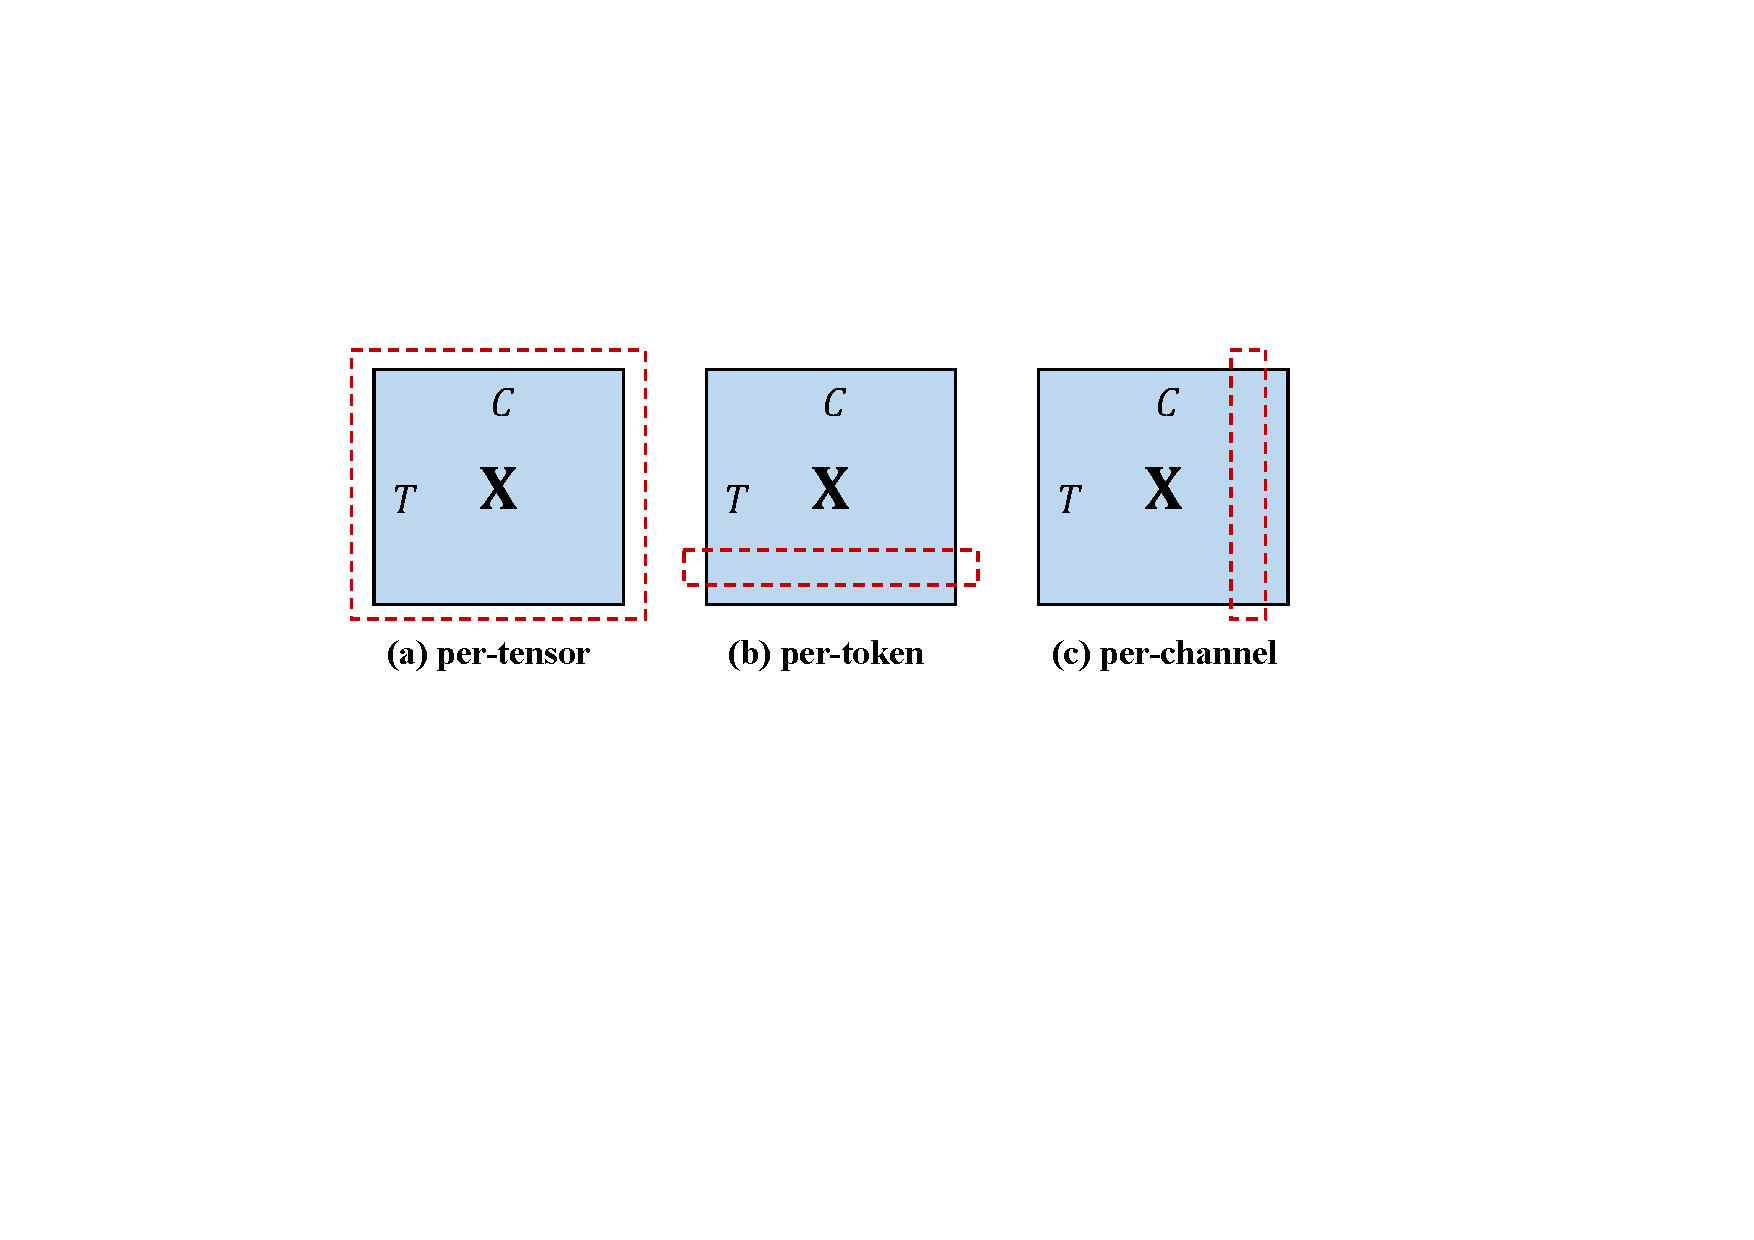
\includegraphics[width=0.88\linewidth]{figures/kv_quant.pdf}
    \caption{Three types of quantization. Then matrix $\mathbf{X} \in \mathbb{R}^{T\times C}$, where $T$ is the number of tokens and $C$ is the feature dimension.}
    \label{fig:kv_quant}
\end{figure}


\subsubsection{Mixed-precision quantization}\label{sssec:kv_quant_mixed_precision}
Unlike fixed-precision quantization, where all Keys or Values are quantized to the same bit-width (e.g., 4-bit or 8-bit), 
mixed-precision quantization assigns higher or full precision to Keys and Values of critical tokens and parts while using lower precision for less critical parts.
The summary of KV mixed-precision quantization is listed in Tab.~\ref{tab:kv_mix_precision}.
KVQuant~\cite{hooper2024kvquant} proposes several strategies to quantize Keys and Values smoothly based on observations.
Firstly, KVQuant observes that the key values exhibit outliers in specific channels prior to applying Rotary Positional Embedding (RoPE).
However, after applying RoPE, the magnitudes of these outlier channels become less consistent, creating a unique challenge for low-precision quantization.
Thus, KVQuant~\cite{hooper2024kvquant} proposes to quantize the Keys per channel before applying the RoPE operations and to quantize the Values per token.
Secondly, KVQuant~\cite{hooper2024kvquant} observes that KV cache activations contain outliers that skew the quantization range. To address this, they isolate outliers per vector (e.g., per-channel or per-token), store them in a sparse format, and quantize the remaining values to a narrower range.
Thirdly, LLMs disproportionately allocate high attention scores to the first token (i.e., attention sink), and quantizing the first token will damage the performance of LLMs.
Thus, KVQuant~\cite{hooper2024kvquant} retains the first token in full precision (FP16) while quantizing the rest of the sequence, which is also used by IntactKV~\cite{liu2024intactkv} and SKVQ~\cite{duanmu2024skvq}.
Similar to KVQuant~\cite{hooper2024kvquant}, KIVI~\cite{liu2024kivi} quantizes the Key cache per-channel, as certain channels exhibit large outliers, and the Value cache per-token,  as there are no significant outlier patterns in the Value cache.
Additionally, KIVI~\cite{liu2024kivi} retains the most recent Keys and Values in full precision, while quantizing older KVs. This approach is based on the observation that the most recent KVs are critical for generating subsequent tokens.


\begin{table*}[t]
\small
\setlength\tabcolsep{2pt}
\centering
\caption{The summary of outlier redistribution models in Sec.~\ref{sssec:outlier_redistribution}.}
\label{tab:outlier_redistribution}
\begin{tabular}{c|c|c|c|c}
\toprule
\textbf{Model} & \textbf{Operation} & \textbf{Formula} & \textbf{Learn} & \textbf{Remarks} \\ \midrule
        MassiveAct.~\cite{DBLP:journals/corr/abs-2402-17762}        &     Add virtual tokens               & $\text{softmax} \left( \frac{\mathbf{Q} \begin{bmatrix} \mathbf{K}^T, & \mathbf{k}' \end{bmatrix}}{\sqrt{d}} \right) 
\begin{bmatrix} \mathbf{V} \\ \mathbf{v}'^T \end{bmatrix}$                 &        \checkmark            &    Learnable $\mathbf{k}'$, $\mathbf{v}'$            \\ \midrule

               
   QuaRot~\cite{ashkboos2024quarot}           &            Hadamard rotation          &  $ \mathbf{XW}^\top = (\mathbf{XH})(\mathbf{H}^\top \mathbf{W}^\top)
$               &          $\times$          &    $\mathbf{H}^\top \mathbf{H} = \mathbf{I}
$             \\ \midrule


   Qserve~\cite{DBLP:journals/corr/abs-2405-04532}            &            Hadamard rotation          &  $ \mathbf{XW}^\top = (\mathbf{XH})(\mathbf{H}^\top \mathbf{W}^\top)
$               &          $\times$          &     $\mathbf{H}^\top \mathbf{H} = \mathbf{I}
$             \\ \midrule


   Q-INT4~\cite{DBLP:conf/nips/XiLCZ23}             &            Hadamard rotation          &  $ \mathbf{XW}^\top = (\mathbf{XH})(\mathbf{H}^\top \mathbf{W}^\top)
$               &          $\times$          &     $\mathbf{H}^\top \mathbf{H} = \mathbf{I}
$             \\ \midrule


               
       SmoothQuant~\cite{DBLP:conf/icml/XiaoLSWDH23}        &     Scaling                &      $  (\mathbf{X} \operatorname{diag}(\mathbf{s})^{-1}) \cdot (\operatorname{diag}(\mathbf{s}) \mathbf{W}^\top)
$            &            $\times$        &    $\mathbf{s} \in \mathbb{R}^{c_i}$              \\ \midrule

               
       QS+~\cite{wei2023outlier}        &    Scaling, Shifting                &      $ ((\mathbf{X}-\mathbf{z}) \operatorname{diag}(\mathbf{s})^{-1} \cdot \operatorname{diag}(\mathbf{s})+\mathbf{z}) \mathbf{W}^\top
$            &         $\times$           &    $\mathbf{s} \in \mathbb{R}^{c_i}$              \\ \midrule


AWQ~\cite{DBLP:conf/mlsys/0002TTYCWXDG024}   &   Scaling                 &       $ \arg\min_{\mathbf{s}} \left\| \mathbf{X}\mathbf{W}^\top - \mathbf{X}\operatorname{diag}(\mathbf{s})^{-1})Q(\operatorname{diag}(\mathbf{s})\mathbf{W}^\top) \right\|$
      &     \checkmark               &  Quantization $Q(\cdot)$                \\ \midrule
      

OmniQuant~\cite{shao2023omniquant}    & Scaling, shifiting                 &   $Q_a\left(\frac{\mathbf{X} - \boldsymbol{\delta}}{\mathbf{s}}\right) Q_w\left(\mathbf{s} \odot \mathbf{W}^\top\right) + \mathbf{B} + \boldsymbol{\delta} \mathbf{W}^\top
$           &       \checkmark               &  Learnable $Q_a(\cdot)$, $Q_w(\cdot)$                 \\ \midrule


      DuQuant~\cite{lin2024duquant}          &        Rotation, permutation            &    $ 
[(\mathbf{X} \cdot \mathbf{\Lambda}) \hat{\mathbf{R}}_{(1)} \cdot \mathbf{P} \cdot \hat{\mathbf{R}}_{(2)}] 
\cdot 
[\hat{\mathbf{R}}_{(2)}^\top \cdot \mathbf{P}^\top \cdot \hat{\mathbf{R}}_{(1)}^\top (\mathbf{\Lambda}^{-1} \cdot \mathbf{W}^\top)]$              &              $\times$      &   Matrices $\mathbf{P}$, $\mathbf{R}$
%permutation and rotation matrices.             
\\ \midrule

    AffineQuant~\cite{ma2024affinequant}           &              Affine transform      &      $\arg\min_{\mathbf{P}} \left\| \mathbf{X}\mathbf{W}^\top - \mathbf{X}\mathbf{P}^{-1} Q(\mathbf{P}\mathbf{W}^\top) \right\|_F^2$            &            \checkmark        &   Quantization $Q(\cdot)$              \\ \midrule

               
    FlatQuant~\cite{sun2024flatquant}    &   Affine transform                  &   AffineQuant +   $\mathbf{P} = \mathbf{P}_1 \otimes \mathbf{P}_2
$            &       \checkmark             & 
Decomposition
%$\operatorname{vec}(\mathbf{V})(\mathbf{P}_1 \otimes \mathbf{P}_2) = \operatorname{vec}(\mathbf{P}_1^\top \mathbf{V} \mathbf{P}_2)$            
\\ \bottomrule        
\end{tabular}
\end{table*}

Similar to KIVI~\cite{liu2024kivi}, WKVQuant~\cite{yue2024wkvquant} temporarily retains the most recent Keys and Values in full precision, while quantizing only the past KV cache. 
This approach helps preserve precision during computation. Additionally, WKVQuant~\cite{yue2024wkvquant} introduces a two-dimensional quantization strategy, which optimizes parameter matrix to align the values in the KV cache into a smoother and more uniform range, significantly improving quantization quality.
GEAR~\cite{kang2024gear}, MiKV~\cite{yang2024no}, ZipCache~\cite{he2024zipcache}  and ZIPVL~\cite{he2024zipvl}  quantize the KV cache based on the importance of each to achieve efficient and effective compression.
First, GEAR~\cite{kang2024gear} applies quantization to compress the majority of less important entries (e.g., 98\%) to ultra-low precision, significantly reducing memory usage. Next, GEAR~\cite{kang2024gear} employs a low-rank matrix to approximate residual errors, capturing structured patterns in the data. Also, GEAR~\cite{kang2024gear} uses a sparse matrix stores outliers, correcting individual errors caused by these values.
MiKV~\cite{yang2024no} is a mixed-precision KV cache quantization approach. Based on the importance of each token, measured using existing methods like H2O~\cite{zhang2023h2o} and SnapKV~\cite{li2024snapkv}, MiKV~\cite{yang2024no} stores less important KV pairs in low precision while retaining the most important KV pairs in high precision.
Instead of approximating the importance weight of each token, ZipCache~\cite{he2024zipcache} accurately computes the importance of each token.
Instead of computing importance score, PrefixQuant~\cite{chen2024prefixquant} observes that token-wise outliers frequently occur at fixed positions (e.g., initial tokens) or low-semantic-value tokens (e.g., ".", "\textbackslash n").
Based on this observation, PrefixQuant~\cite{chen2024prefixquant} identifies high-frequency outlier tokens in LLMs offline and prefixes them in the KV cache, effectively eliminating token-wise outliers.
Similarly, MiniKV~\cite{sharma2024minikvpushinglimitsllm} observes that important tokens can be identified before generation and remain consistent throughout the generation process, retaining these important tokens in high precision.



QAQ~\cite{dong2024qaq} proposes a quality adaptive quantization approach to dynamically determine the suitable quantization bit for each token, based on its importance and sensitivity, while handling outliers and exceptions to maintain model performance.
SKVQ~\cite{duanmu2024skvq} introduces the clipped dynamic quantization with channel reorder. First,  SKVQ~\cite{duanmu2024skvq} uses a transformation-invariant permutation to group similar channels based on their statistical characteristics and applies clipped dynamic quantization to mitigate the outlier problem. Second,  SKVQ~\cite{duanmu2024skvq} maintains high precision for the initial tokens and the most recent tokens while quantizing older tokens. Consequently, SKVQ~\cite{duanmu2024skvq} effectively reduces quantization errors and improves the accuracy of the quantized model.
CacheGen~\cite{liu2024cachegen} and AsymKV~\cite{tao2024asymkv} use layer-wise asymmetric quantization, assigning higher-bit precision  to key matrices in sensitive early layers and lower-bit precision  to less sensitive layers, balancing memory efficiency and performance.
Particularly,
CacheGen~\cite{liu2024cachegen}  also exploits token-wise locality by encoding deltas (differences) between KV tensors of nearby tokens instead of raw values.
Atom~\cite{zhao2024atom} identifies and separates outlier channels, reordering the matrix to group these outlier channels at the end, thereby ensuring regular memory access patterns for improved hardware utilization.
Then, Atom~\cite{zhao2024atom} quantizes outliers with higher precision, while normal channels are quantized to INT4 for maximum efficiency. 
In particular, Atom~\cite{zhao2024atom} applies fine-grained group quantization by dividing matrices into smaller subgroups (e.g., 128 elements per group) and performing quantization independently within each group.







\subsubsection{Outlier Redistribution }\label{sssec:outlier_redistribution}
As previously mentioned, outliers in the Keys and Values present significant challenges for their quantization. Recent research has proposed two main approaches to address this issue: redistributing the outliers into newly appended virtual tokens or applying equivalent transformation functions to smooth the Keys and Values for improved quantization accuracy.
The summary of existing outlier redistribution models are listed in Table.~\ref{tab:outlier_redistribution}.


Specifically, MassiveActivation~\cite{DBLP:journals/corr/abs-2402-17762} highlights the phenomenon of massive activations in large language models (LLMs), where a small subset of activations is exponentially larger than the rest. To address this, MassiveActivation~\cite{DBLP:journals/corr/abs-2402-17762} proposes appending a virtual token to the inputs, allowing LLMs to encapsulate the massive outliers within these learned keys and values for each head.
Then, we introduce the  equivalent transformation function-based approaches. Firstly,
QuaRot~\cite{ashkboos2024quarot}, Qserve~\cite{DBLP:journals/corr/abs-2405-04532}, and Q-INT4~\cite{DBLP:conf/nips/XiLCZ23} redistributes outlier values across all channels by Hadamard rotation, successfully lowering the maximum value of outlier tokens. 
The Hadamard rotation of activations can be incorporated into the preceding linear layer, thereby redistributing the outliers of Keys and Values into the parameters.
Despite this improvement, outlier tokens still exhibit magnitudes hundreds of times greater than normal tokens, causing notable performance issues when using shared quantization scales across tokens~\cite{chen2024prefixquant}.
Expanding on this idea, SpinQuant~\cite{liu2024spinquant} proposes training an orthogonal matrix instead of relying on a random Hadamard matrix to achieve better performance. Similarly, DuQuant~\cite{lin2024duquant} employs channel permutation to evenly distribute outliers across blocks and utilizes block rotation to further smooth outliers.  



SmoothQuant~\cite{DBLP:conf/icml/XiaoLSWDH23} leverages a key observation that different tokens show similar patterns of variation across their channels. Based on this insight, it strategically shifts the quantization complexity from activations to weights through an offline process.
Specifically, SmoothQuant~\cite{DBLP:conf/icml/XiaoLSWDH23} introduces a mathematically equivalent per-channel scaling transformation:
$\mathbf{Y} = (\mathbf{X}\text{diag}(\mathbf{s})^{-1}) \cdot (\text{diag}(\mathbf{s})\mathbf{W}) = \mathbf{\hat{X}}\mathbf{\hat{W}}$
where $\mathbf{X}$ represents Keys or Values, and the smoothing factor $\mathbf{s}\in \mathbb{R}^{C_i}$ is used to scale $\mathbf{X}$. This transformation achieves two key benefits: it smooths the distribution of Keys and Values to facilitate easier quantization, and it allows the smoothing factors to be efficiently incorporated into the parameters of previous layers during offline processing.
In particular, the smooth factor $\mathbf{s}$ is dynamically decided on based on inputs.
Similarly,
The OS+~\cite{wei2023outlier} introduces channel-wise shifting to eliminate outlier asymmetry and channel-wise scaling to reduce outlier concentration. These operations are seamlessly migrated to subsequent layers, maintaining equivalence with the floating-point model while improving quantization performance.
%DuQuant~\cite{lin2024duquant}ntroduces a dual transformation approach using rotation and permutation matrices to redistribute activation outliers for efficient quantization.



Instead of using handcrafted transformations~\cite{lin2024duquant,wei2023outlier,DBLP:conf/icml/XiaoLSWDH23} to shift the quantization difficulty from activations to weights,
AffineQuant~\cite{ma2024affinequant}
uses an affine transformation matrix that combines both scaling and rotation transformations. 
This allows it to optimize weight distributions more effectively, aligning them better with the quantization function and reducing quantization errors.
The affine transformation matrix provides richer flexibility compared to SmoothQuant’s scalar-based scaling, enabling finer adjustments to the weight and activation distributions.
Based on AffineQuant~\cite{ma2024affinequant},
FlatQuant~\cite{sun2024flatquant} introduces a fast and learnable affine transformations to enhance the flatness of weights and activations, which decomposes transformations into smaller matrices to reduce memory and computational costs.
Similarly,
AWQ~\cite{DBLP:conf/mlsys/0002TTYCWXDG024} and 
OmniQuant~\cite{shao2023omniquant} proposes
differentiable and learnable equivalent transformations, 
which optimize the equivalent parameters (e.g., channel-wise scaling and shifting) in an end-to-end manner using gradient descent.

\subsubsection{Summary and Future Directions}
KV cache quantization is a crucial technique for reducing memory and computational overhead in large language models (LLMs) during autoregressive decoding. While significant progress has been made, this field remains dynamic and rapidly evolving, with several promising directions for future research.
Firstly,
one promising avenue is the development of real-time adaptive quantization methods. These techniques could dynamically adjust quantization levels during inference based on real-time metrics such as token importance, outlier presence, or sequence length. Such an approach could significantly enhance efficiency while maintaining performance, especially for processing long sequences with varying levels of complexity.
Secondly,
another important direction is extending KV cache quantization to multi-modal and multi-task models. Multi-modal models, which process inputs from diverse domains such as text, vision, and audio, and multi-task scenarios often exhibit highly diverse attention patterns and memory demands. This necessitates the design of more advanced and tailored quantization strategies to balance efficiency and accuracy in these increasingly complex settings.

Thirdly,
hybrid quantization techniques also hold significant potential. By combining fixed-precision, mixed-precision, and outlier redistribution methods, researchers could develop more versatile and efficient quantization frameworks. For instance, integrating mixed-precision allocation schemes with outlier smoothing transformations could optimize both memory usage and performance, offering a flexible approach adaptable to a variety of tasks and models.
finally, addressing the challenge of outliers remains a critical area of focus. Outliers can have a disproportionate impact on quantization efficiency and model performance. Future research could explore advanced outlier detection mechanisms or innovative encoding techniques to mitigate their effects. Improved handling of outliers could further enhance the effectiveness of quantization methods, enabling more robust and memory-efficient implementations.




\subsection{KV Cache Low-rank Decomposition}\label{ssec:kv_low_rank}
Existing studies have demonstrated that the majority of information within KV caches can be captured by a small subset of their singular values or low-rank components, making low-rank decomposition a powerful tool for compression. 
By leveraging this property, KV cache low-rank decomposition techniques aim to reduce memory requirements while preserving the essential information required for accurate attention computations.
Low-rank decomposition strategies can be classified into three main approaches: \textbf{Singular Value Decomposition (SVD)}, which exploits the low-rank structure of KV matrices to retain the most critical singular values; 
\textbf{Tensor Decomposition}, which factorizes KV matrices into smaller components for minimal redundancy; 
and \textbf{Learned Low-rank Approximation}, which incorporates adaptive mechanisms to optimize compression based on learned representations. 
Each method provides a unique balance of computational efficiency and accuracy retention, enabling scalable and memory-efficient LLM inference.



\subsubsection{Singular Value Decomposition}\label{sssec:kv_low_rank_svd}
Firstly, 
ECKVH~\cite{yu2024effectively}, EigenAttention~\cite{saxena2024eigen}, and ZDC~\cite{zhang2024zero} shows that KV caches have a low-rank property, where a small number of top singular values retain most of the information. Using Singular Value Decomposition (SVD), the method compresses KV caches by grouping heads, applying SVD, and retaining top singular values, effectively reducing the number of KV heads with minimal error.
Also, ZDC~\cite{zhang2024zero} uses an adaptive hybrid compression ratio mechanism to assign higher compression to unimportant tokens in shallower layers while preserving more important tokens in deeper layers, leveraging the similarity of token characteristics in adjacent layers.
Secondly, rather than decomposing KV pairs, LoRC~\cite{zhang2024lorc} employs a low-rank approximation of KV weight matrices and adopts a progressive compression strategy to efficiently compress KV caches without requiring model retraining.
Specifically,
LoRC~\cite{zhang2024lorc} uses SVD to compress the Keys and Values parameter matrices (i.e., $\mathbf{W}^k_i$ and $\mathbf{W}^v_i$) as  $\mathbf{W}^k_i=\mathbf{U}^k_i \mathbf{\Sigma}^k_i {\mathbf{P}^k_i}^\top$ and $\mathbf{W}^v_i=\mathbf{U}^v_i \mathbf{\Sigma}^v_i {\mathbf{P}^v_i}^\top$.
Also, compression is applied conservatively in shallower layers to minimize error amplification and more aggressively in deeper layers.
Then, instead of storing $\mathbf{K}^i=\mathbf{X}_i\mathbf{W}^k_i$ and $\mathbf{V}^i=\mathbf{X}_i\mathbf{W}^v_i$, it only stores $\mathbf{\hat{K}}^i=\mathbf{X}_i\mathbf{U}^k_i$ and $\mathbf{\hat{V}}^i=\mathbf{X}_i\mathbf{U}^v_i$, along with $ \mathbf{\Sigma}^k_i {\mathbf{P}^k_i}^\top$ and $ \mathbf{\Sigma}^v_i {\mathbf{P}^v_i}^\top$.
Also, ShadowKV~\cite{sun2024shadowkv} performs SVD decomposition directly on pre-RoPE keys to reduce the dimensionality of the key representations.
Palu~\cite{chang2024palu} applies SVD to compress both Keys and Values.





\subsubsection{Tensor Decomposition}\label{sssec:kv_low_rank_tensor}
Tensor decomposition~\cite{kuleshov2015tensor, zhou2017tensor,haeffele2015global} is a widely used algorithm for factorizing a matrix into a sequential product of local tensors, such as Matrix Product Operator (MPO)~\cite{liu2021enabling} and turker decomposition~\cite{malik2018low} .
Taking Matrix Product Operator (MPO)~\cite{liu2021enabling} as an example, the decomposition of a matrix $\mathbf{W} \in \mathbb{R}^{I \times J}$ using MPO can be  defined as:
\begin{equation}\label{eq:mpo}
    \text{TD}(\mathbf{W}) = \prod_{k=1}^n \mathcal{T}_{(k)}[d_{k-1}, i_k, j_k, d_k],
\end{equation}
where $\mathcal{T}_{(k)}$ represents the local tensor of size $d_{k-1} \times i_k \times j_k \times d_k$, with $\prod_{k=1}^n i_k = I$ and $\prod_{k=1}^n j_k = J$. Here, $n$ denotes the number of local tensors, collectively referred to as the decomposed tensors.
As shown in Eaquation~\eqref{eq:mpo},
MPO-based tensor decomposition is well-suited for KV cache compression as it reduces the memory footprint by factorizing large key and value matrices into smaller local tensors, enabling efficient storage while preserving essential information. This approach minimizes redundancy and maintains the structural integrity required for accurate attention computations.
DecoQuant~\cite{liu2024unlocking} combines quantization with low-rank decomposition to effectively reduce quantization errors. Specifically, DecoQuant~\cite{liu2024unlocking} leverages the Matrix Product Operator (MPO) to decompose matrices into smaller local tensors. The larger tensors, which contain most of the parameters, are quantized to low-bit precision, while the smaller tensors retain high precision to minimize overall quantization error.

\subsubsection{Learned Low-rank Approximation}\label{sssec:kv_low_rank_learned}
LESS~\cite{dong2024get} introduces a novel {learned-kernel-based low-rank approximation} approach to efficiently approximate the results of the softmax function. Specifically, LESS~\cite{dong2024get} replaces the softmax with a {separable similarity metric}, \(\phi(\mathbf{q}_t) \psi(\mathbf{K}_t)^\top\), where \(\phi\) and \(\psi\) are row-wise functions. Here, \(\mathbf{q}_t \in \mathbb{R}^{1 \times D}\) represents the query, and \(\mathbf{K}_t \in \mathbb{R}^{t \times D}\) represents the keys at step \(t\).
To elaborate, if \(\phi\) and \(\psi\) are such that:
$a_t = \text{softmax} \left( \frac{\mathbf{q}_t \mathbf{K}_t^\top}{\sqrt{D}} \right) \mathbf{V}_t 
\approx \frac{\phi(\mathbf{q}_t) \psi(\mathbf{K}_t)^\top \mathbf{V}_t}{\phi(\mathbf{q}_t) \psi(\mathbf{K}_t)^\top \mathbf{1}_{S \times 1}}$,
then we only need to cache the {hidden states} \(\mathbf{H}_t = \psi(\mathbf{K}_t)^\top \mathbf{V}_t \in \mathbb{R}^{R \times D}\) and the {normalization factor} \(\mathbf{z}_t = \sum_{s=1}^t \psi([\mathbf{K}_t]_s) \in \mathbb{R}^{1 \times R}\) for inference.
Similarly,
MatryoshkaKV~\cite{linMatryoshkaKVAdaptiveKV2024} 
compresses KV caches along the feature dimension by leveraging trainable orthogonal projection matrices.


\subsubsection{Summary and Future Directions}
KV cache low-rank decomposition is a powerful technique for compressing KV caches in LLMs while maintaining the quality of attention computations. Current methods primarily rely on fixed low-rank approximations applied uniformly across all layers or tokens. However, future advancements could focus on dynamic rank adjustment, where the rank is tailored based on token importance, sequence length, or layer-specific properties, enabling a more optimal balance between memory efficiency and performance.
Additionally, real-time or streaming applications present a promising avenue for exploration. Since KV caches grow dynamically during inference, lightweight and incremental decomposition methods that can adapt efficiently to expanding sequences will be critical for supporting such scenarios without compromising latency or accuracy.





 
